\chapter{Interferometric stabilisation of reservoir cavity}

\label{ch-stabilisation}

%%%%%%%%%% INTRODUCTION %%%%%%%%%%

\section{Introduction}

In this introductory section, the concept of interferometry is presented. As the name of the chapter suggests, this technique is used to stabilise the reservoir cavity. The reason why an optical cavity needs stabilisation will appear clearer later, but basically, this is due to the fact that light is a wave and that it can interfere with itself inside the cavity. The interferences can be constructive, destructive, or can behave in any intermediate way. Moreover, it will be shown that the interferometric properties are wavelength dependent. Since several wavelengths coexist inside the reservoir, this gives a first glimpse on the complexity entailing its stabilisation. To gain some insight on interferometry, and before moving on to the study of an actual ring cavity, the features of the well known \gls{fp} interferometer are recalled. After that, it is shown that the properties studied for the \gls{fp} can be translated to ring cavities with close to no modification. Finally, under the light of the basic notions of interferometry developed, the difficulties linked to the stabilisation of the reservoir cavity, which is at the heart of the scheme introduced in this thesis, are presented.

%%% FABRY-PEROT INTERFEROMETER %%%

\subsection{Fabry-Perot interferometer}

The \gls{fp} plays an important role in modern optics as it is really ubiquitous. This can be explained by the fact that, despite its great simplicity, it can reach good performance using high reflectivity mirrors, which can be produced using nowadays technologies. In practice, a \gls{fp} cavity is simply made of two facing mirrors as can be viewed on figure \ref{fp}. On this figure, one can see the two mirrors, represented by the vertical black lines, and the different electric fields. The resonance condition, namely the regime where the transmitted electric field $E_{\text{t}}$ is maximum, can be seen intuitively as a situation where the intra-cavity field $E_1$ is in phase with the incident field $E_{\text{in}}$, which leads to the build up of a very intense intra-cavity electric field. On the other hand, the anti-resonance condition is met when $E_{\text{in}}$ and $E_1$ are out of phase. The transmissivity of the \gls{fp} interferometer, which is defined as the ratio $|E_{\text{t}}|^2/|E_{\text{in}}|^2$, is given by \cite{Perot1899}:

\begin{equation}
	\mathcal{T} = \frac{1}{1+\mathcal{F}\sin^2{\left(\frac{\delta \omega}{\text{FSR}}\right)}}
\end{equation}

By using the conservation of energy argument, the reflectivity of the cavity, which is defined as the ratio $|E_{\text{ref}}|^2/|E_{\text{in}}|^2$, reads:

\begin{equation}
	\mathcal{R} = 1 - \mathcal{T}
\end{equation}



\begin{figure}[h]
	\centering
	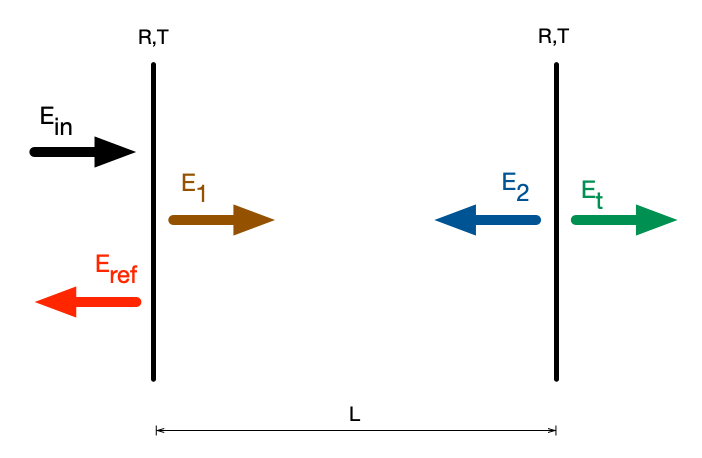
\includegraphics[width=.7\textwidth]{fp}
	\caption{Schematic representation of a \acrlong{fp} interferometer. $E_{\text{in}}$ is the incident electric field, $E_{\text{ref}}$ is the reflected electric field, $E_{\text{t}}$ is the transmitted electric field, $E_{1}$ is the intra-cavity electric field propagating from left to right, $E_{2}$ is the intra-cavity electric field propagating from right to left, $R$ and $T$ are the reflectivity and transmissivity of the mirrors and $L$ is the distance between them.}
	\label{fp}
\end{figure}

\begin{figure}[h]
	\centering
	\begin{subfigure}{.5\textwidth}
		\centering
		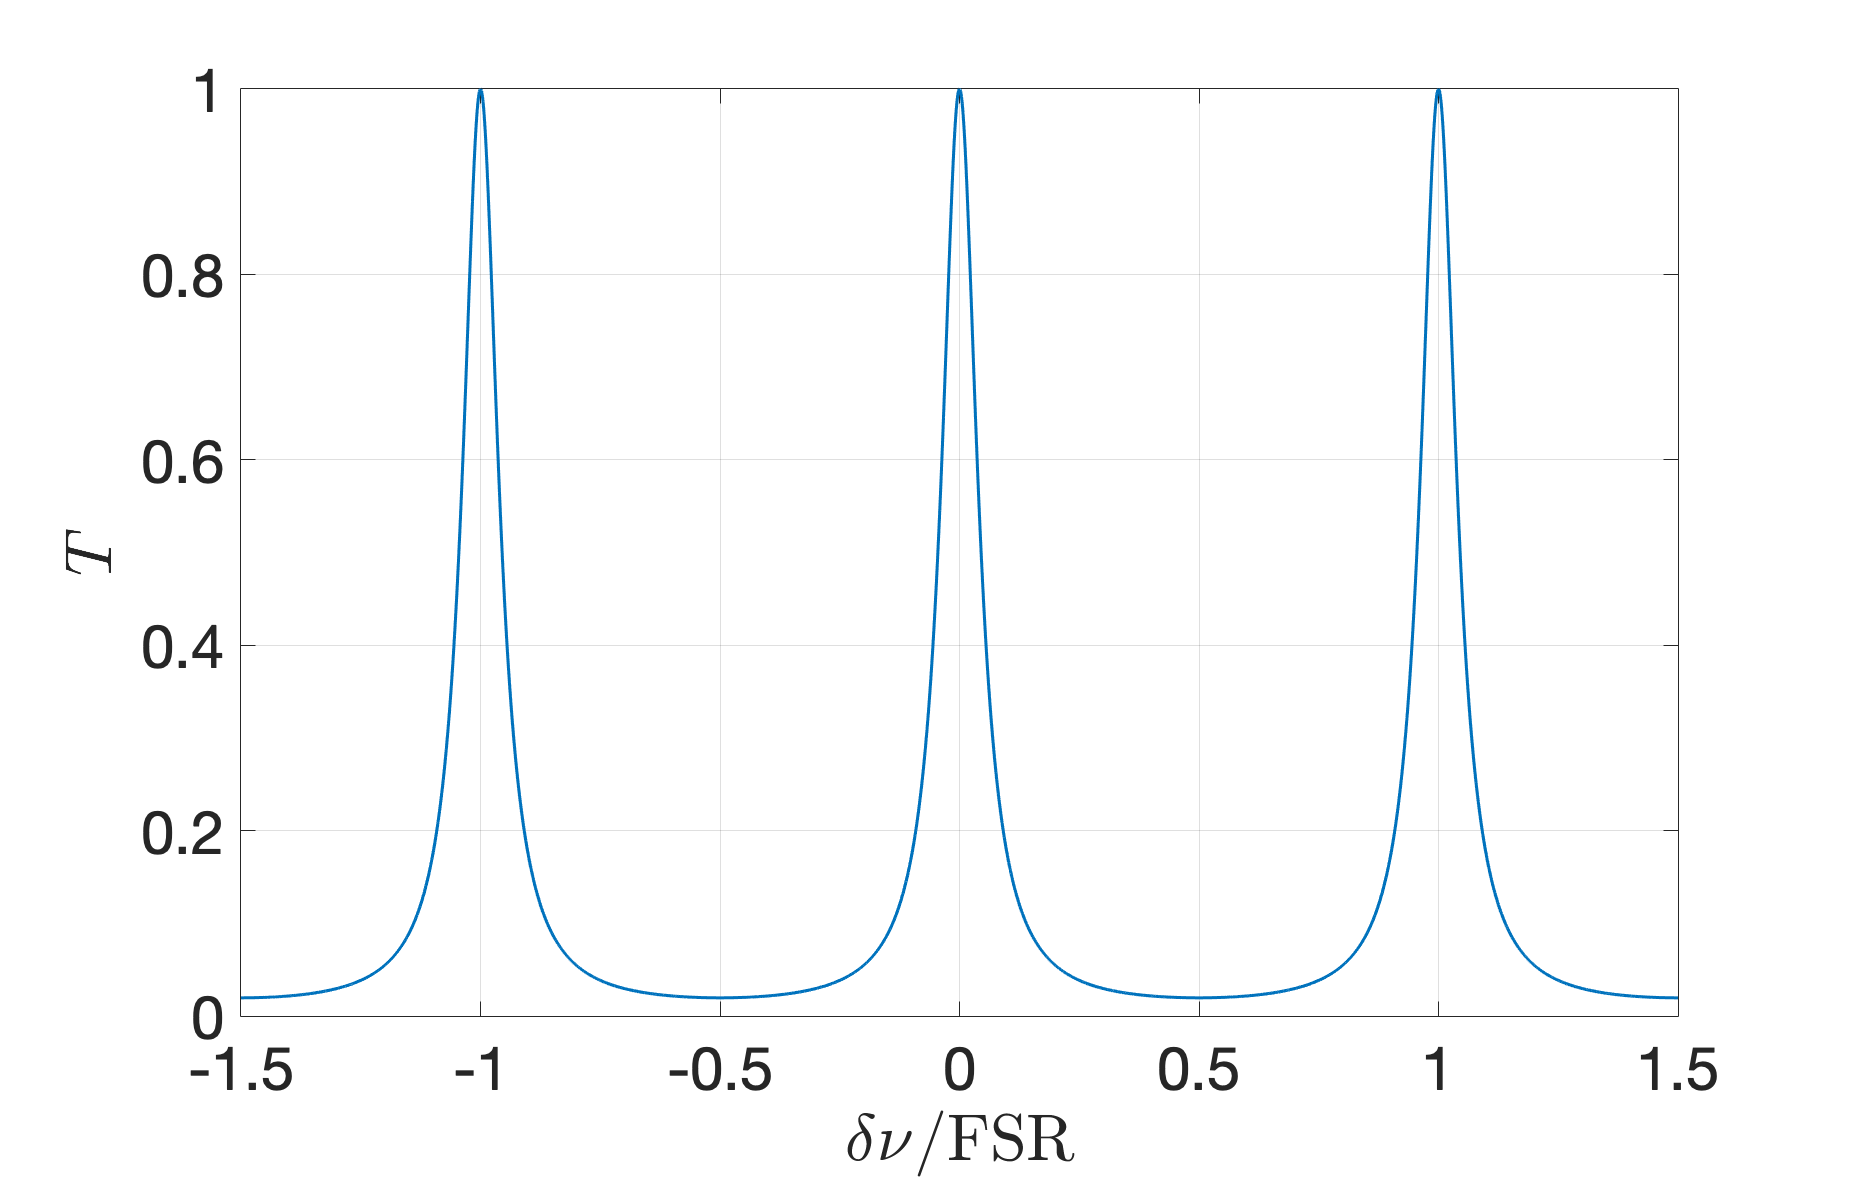
\includegraphics[width=\textwidth]{fp-trans-tf}
	\end{subfigure}%
	\begin{subfigure}{.5\textwidth}
		\centering
		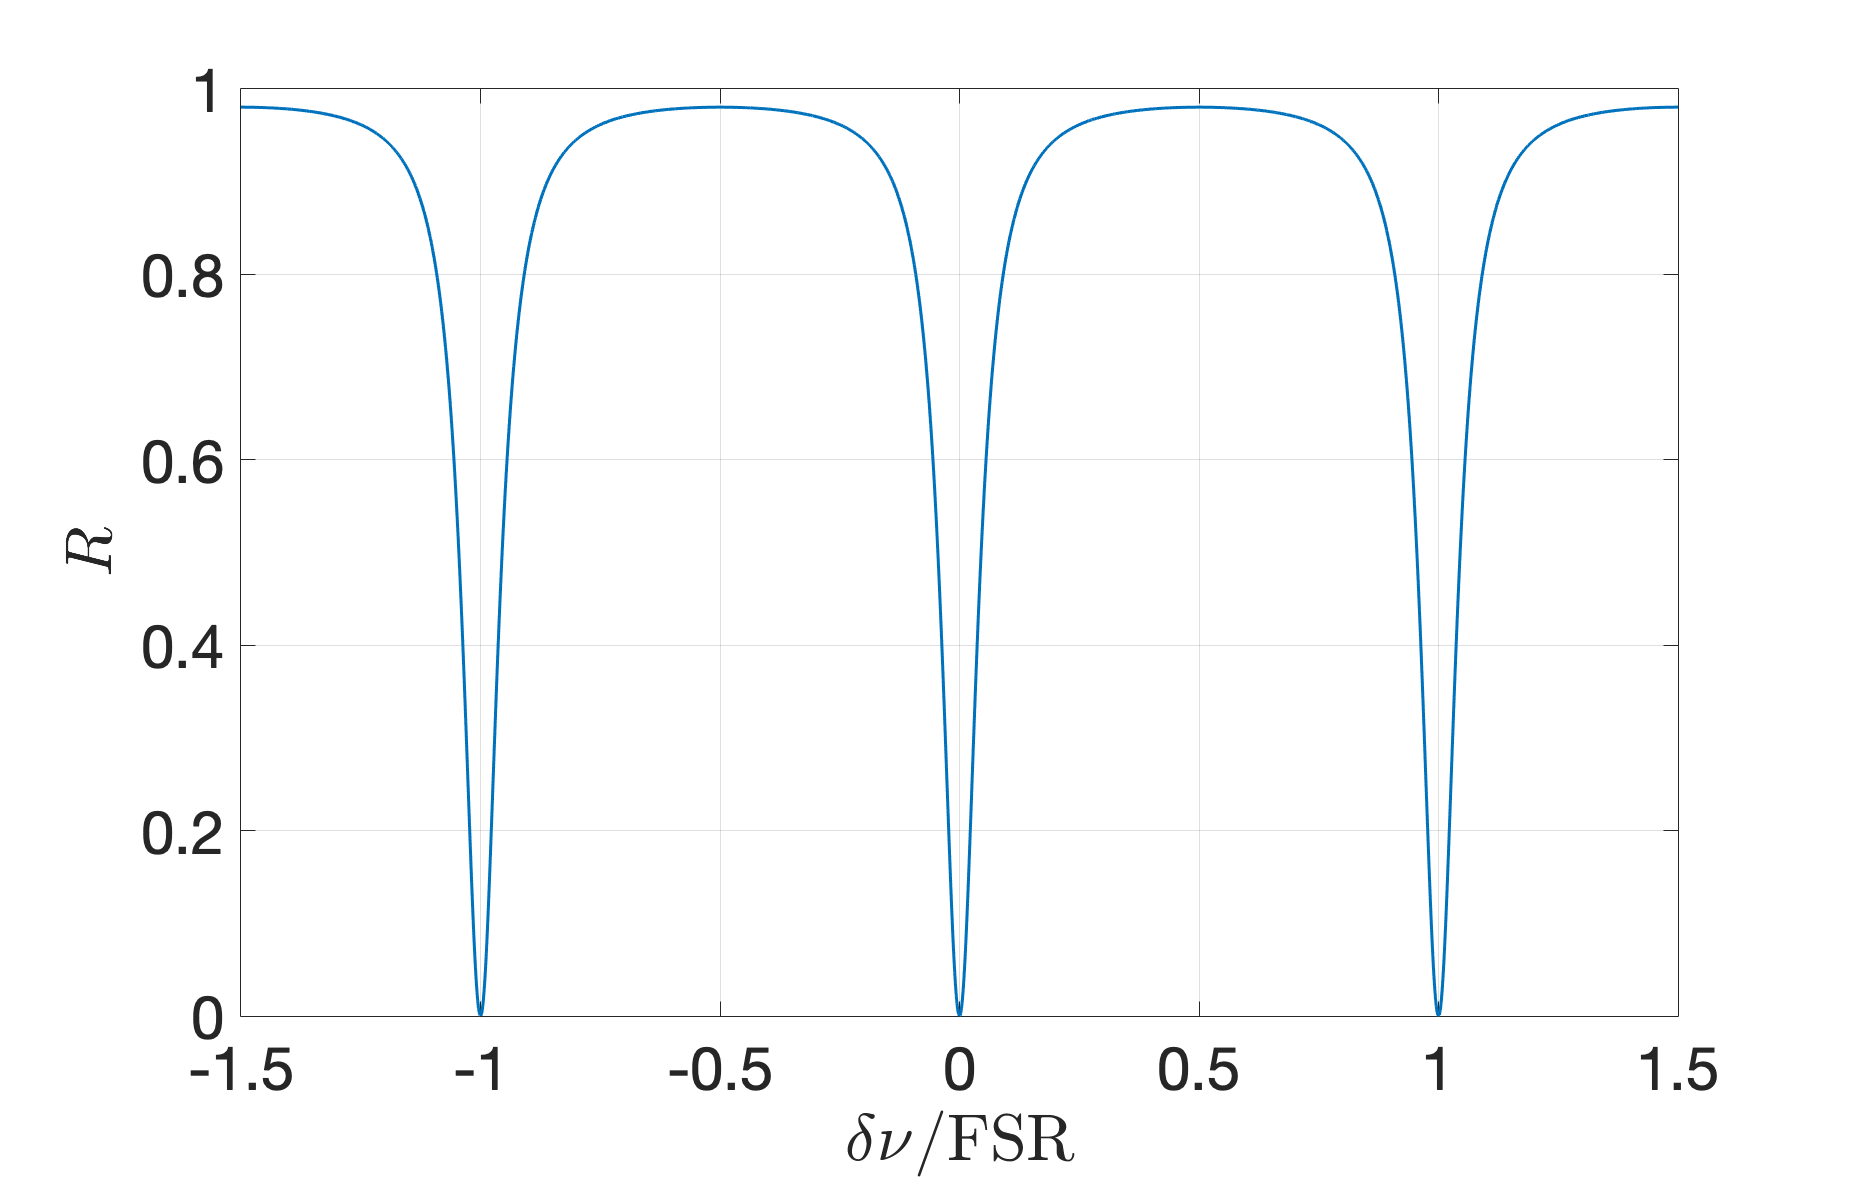
\includegraphics[width=\textwidth]{fp-ref-tf}
	\end{subfigure}
	\caption{Transmissivity $\mathcal{T}$ (left) and reflectivity $\mathcal{R}$ (right) of the cavity. Finesse $\mathcal{F}=50$. }
	\label{fp-tf}
\end{figure}

%%% RING CAVITY INTERFEROMETER %%%

\subsection{Ring cavity interferometer}

\begin{figure}[h]
	\centering
	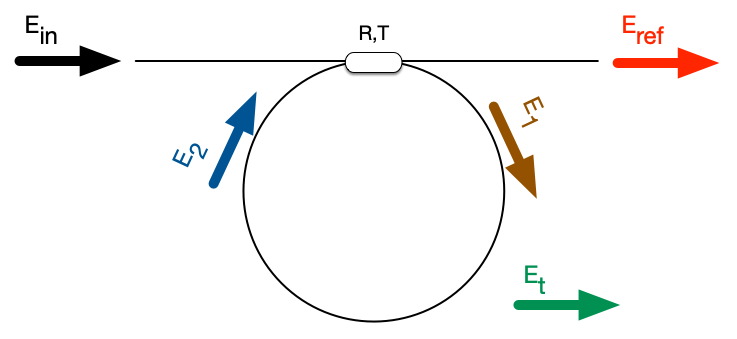
\includegraphics[width=.7\textwidth]{cavity_vs_fb}
	\caption{Schematic view of an optical cavity}
\end{figure}

%%% Challenge %%%

\subsection{Challenge}

%%%%%%%%%% EXPERIMENTAL SETUP %%%%%%%%%%

\section{Experimental setup}

% Mention only one PD

\begin{figure}[h]
	\centering
	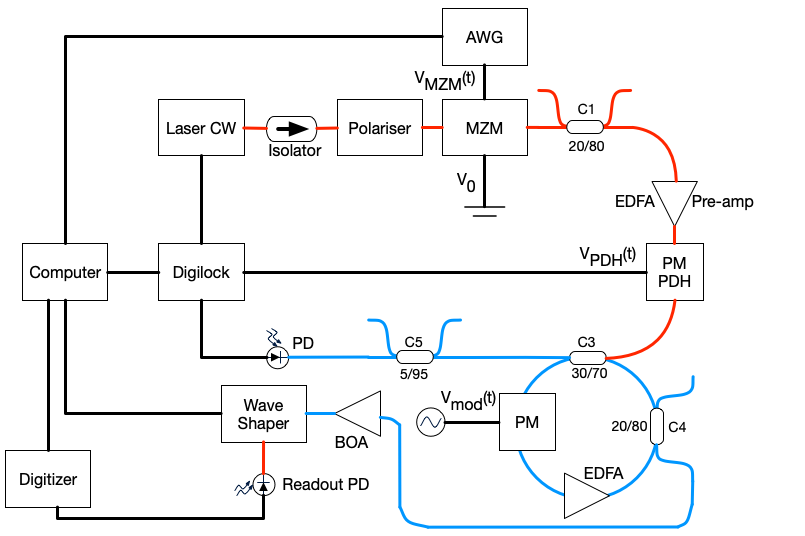
\includegraphics[width=\textwidth]{exp-setup}
\end{figure}

%%%%%%%%%% CHARACTERISATION OF THE RESERVOIR %%%%%%%%%%

\section{Characterisation of the reservoir}

%%% INTRODUCTION %%%

\subsection{Introduction}

%%% TRANSFER FUNCTION OF THE CAVITY %%%

\subsection{Transfer function of the cavity}

% MATHEMATICAL MODEL %

\subsubsection{Mathematical model}

% SIMULATIONS %

\subsubsection{Simulations}

% EXPERIMENTAL RESULTS %

\subsubsection{Experimental results}

%%% EFECTIVE LOSSES %%%

\subsection{Effective losses}

%%% MODULATION DEPTH %%%

\subsection{Modulation depth}

%%%%%%%%%% PDH STABILISATION TECHNIQUE %%%%%%%%%%

\section{Pound-Drever-Hall stabilisation technique}

%%% INTRODUCTION %%%

\subsection{Introduction}

%%% ERROR FUNCTION %%%

\subsection{Error function}

% MATHEMATICAL MODEL %

\subsubsection{Mathematical model}

% SIMULATION %

\subsubsection{Simulation}

% EXPERIMENTAL RESULTS %

\subsubsection{Experimental results}

%%%%%%%%%% CHARACTERISATION OF THE STABILISATION PERFORMANCE FOR DIFFERENT REGIMES %%%%%%%%%%

\section{Characterisation of the stabilisation performance for different regimes}

%%% INTRODUCTION %%%

\subsection{Introduction}

%%% APPROACH %%%

\subsection{Approach}

%%% RESULTS %%%

\subsection{Results}